\documentclass[landscape, a3paper]{article}
\usepackage{tikz}
\usepackage{geometry}
\usetikzlibrary{positioning, shapes.geometric, patterns,shapes,arrows,positioning,calc,arrows.meta}

% Adjust the page layout with the geometry package
\geometry{left=1.5cm, right=1.5cm, top=1.5cm, bottom=1.5cm}

\begin{document}
\begin{figure}
    \centering
    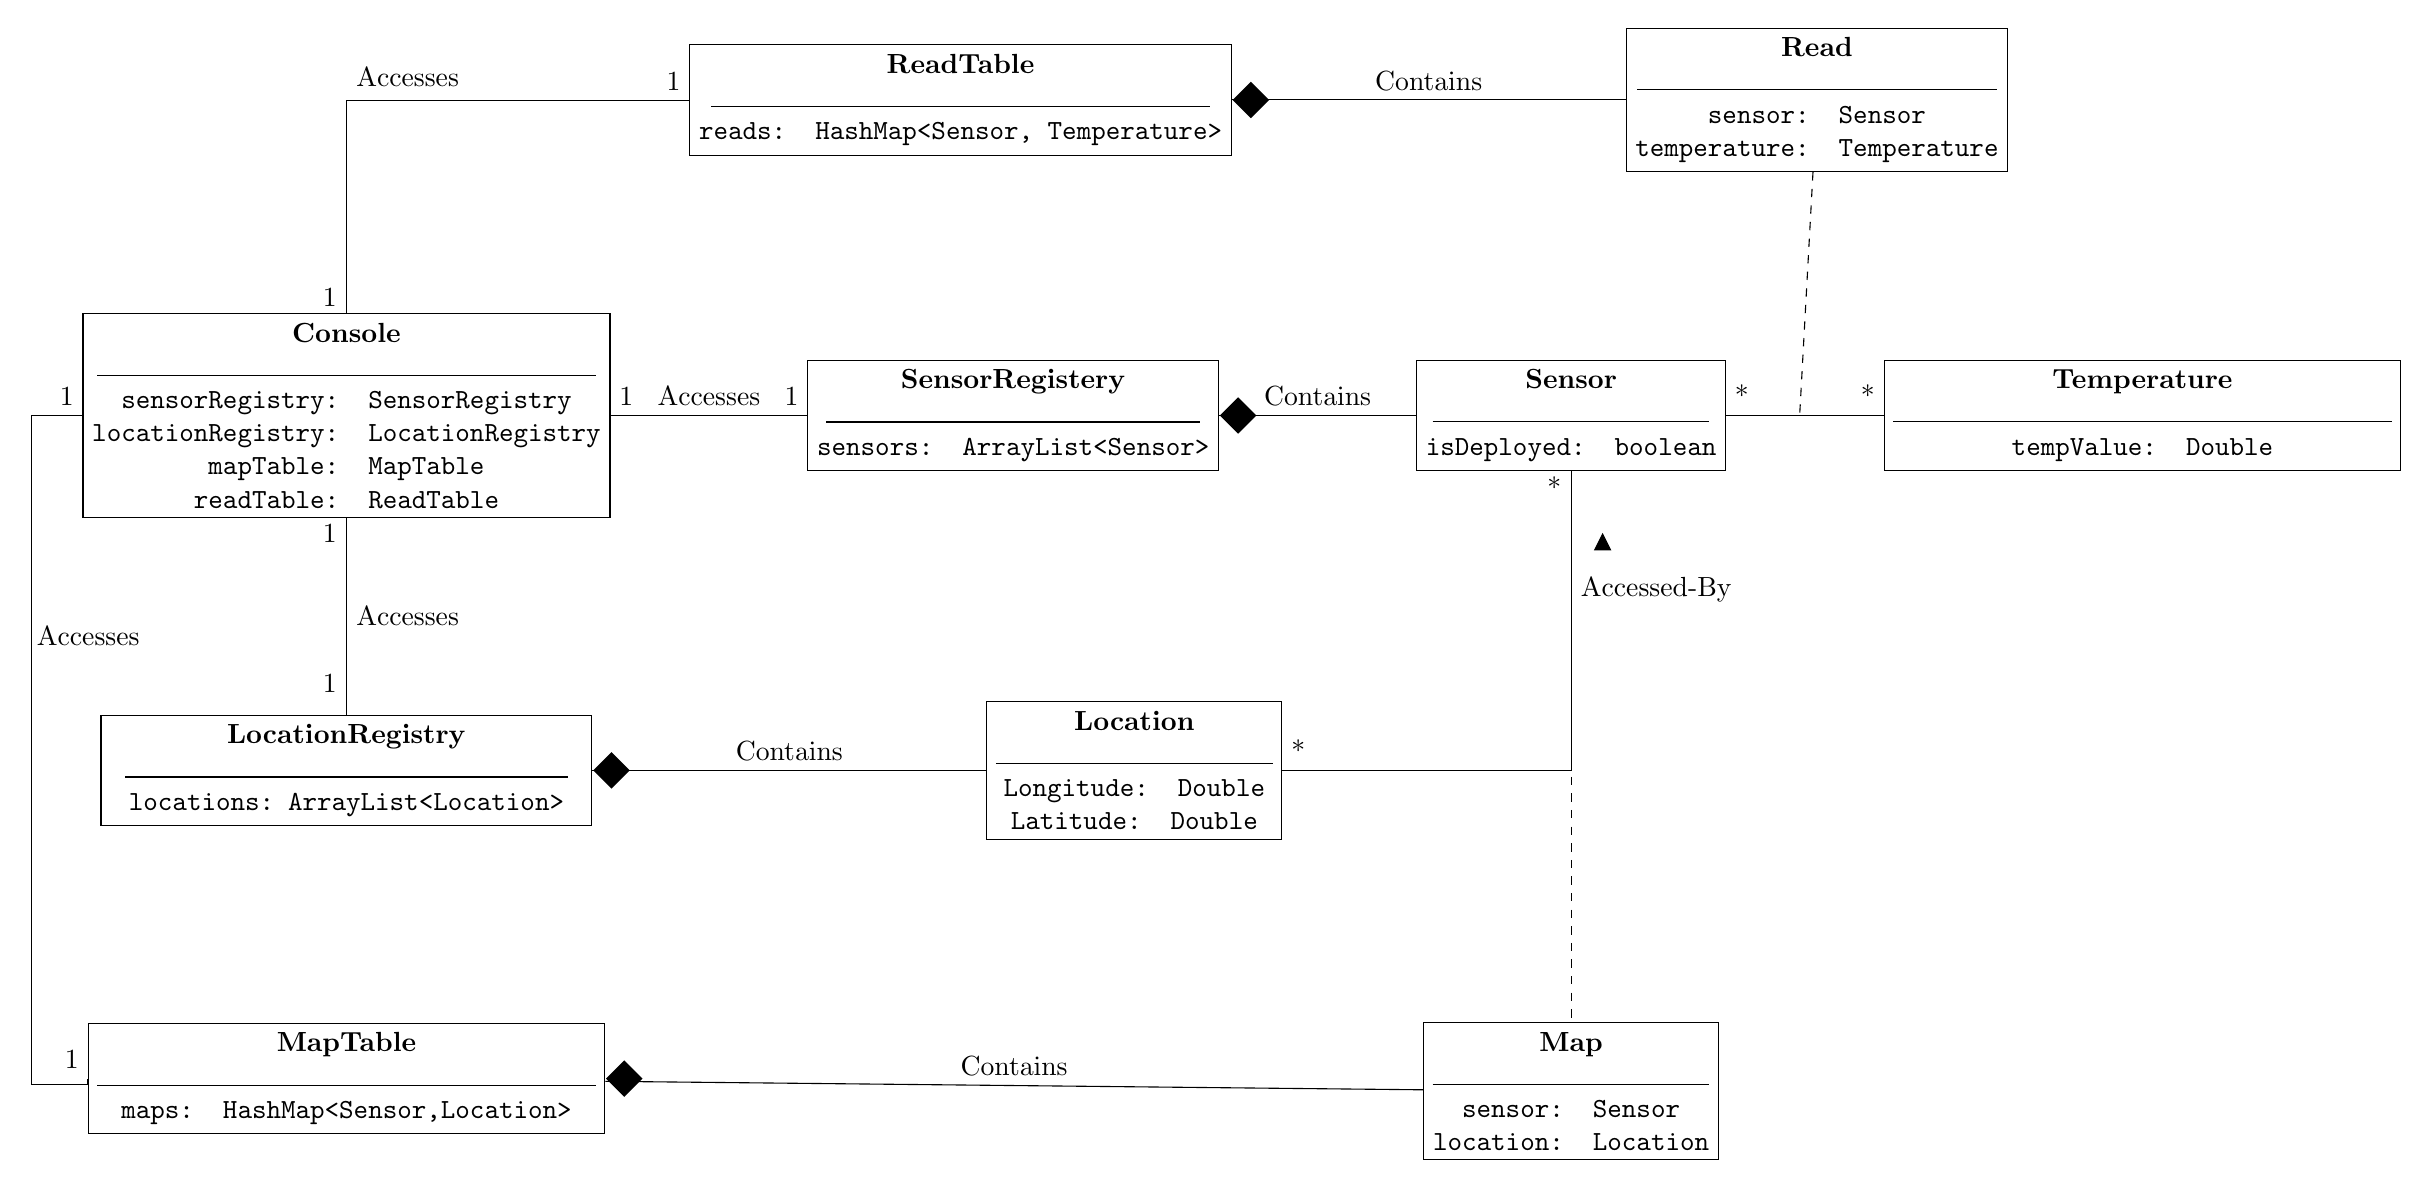
\begin{tikzpicture}[node distance=3cm]
        %-----Entities-----
        
        % Console Entity
        \node [rectangle, draw, align=center] (console) {%
            \textbf{Console} \\
            \line(1,0){180} \\
            \texttt{sensorRegistry: SensorRegistry} \\
            \texttt{locationRegistry: LocationRegistry} \\
            \texttt{mapTable: MapTable} \\
            \texttt{readTable: ReadTable}
        };

        % Location Registry Entity
        \node [rectangle, draw, below=2.5cm of console, align=center, text width=6cm] (lreg) {%
    			\textbf{LocationRegistry} \\
    			\line(1,0){160} \\
    			\texttt{locations: ArrayList<Location>} \\
};

        % Sensor Registry Entity
        \node [rectangle, draw, right=2.5cm of console, align=center] (sreg) {%
            \textbf{SensorRegistery}\\
            \line(1,0){135} \\
            \texttt{sensors: ArrayList<Sensor>}
        }; 
        
        % Sensor Class
        \node [rectangle, draw, right=2.5cm of sreg, align=center] (sensor) {%
            \textbf{Sensor} \\
            \line(1,0){100} \\
            \texttt{isDeployed: boolean}
        };

        % Location Entity
        \node[rectangle, draw, right=5cm of lreg, align=center] (loc) {%
            \textbf{Location} \\
            \line(1,0){100} \\
            \texttt{Longitude: Double} \\
            \texttt{Latitude: Double}
        };


        % Map Table Entity
        \node [rectangle, draw, below=2.5cm of lreg, align=center] (mapt) {%
            \textbf{MapTable}  \\
            \line(1,0){180} \\
            \texttt{maps: HashMap<Sensor,Location>}
        };
        
         % Map Entity
        \node [rectangle, draw, below=7cm of sensor, align=center] (map) {%
            \textbf{Map}  \\
            \line(1,0){100} \\
            \texttt{sensor: Sensor} \\
            \texttt{location: Location}
        };
        
        % Read Table Entity
        \node [rectangle, draw, above right=2cm and 1cm of console, align=center] (readt) {%
            \textbf{ReadTable} \\
            \line(1,0){180} \\
            \texttt{reads: HashMap<Sensor, Temperature>}
        };
        % Read Entity
        \node [rectangle, draw, right=5cm of readt, align=center] (read) {%
            \textbf{Read} \\
            \line(1,0){130} \\
            \texttt{sensor: Sensor} \\
            \texttt{temperature: Temperature}
        };
        
        % Temperature Entity
        \node[rectangle, draw, right=2cm of sensor, align=center] (temp) {%
            \textbf{Temperature} \\
            \line(1,0){180} \\
            \texttt{tempValue: Double}
        };
        
        
        %-----Associations and Cardinality-----
       
        % Connect Console to Map Table
        \draw[-] (console.west)  -- (-4, 0) -| (-4, -8.5) -| (mapt.west) node[left=0.2cm of console,above]{1} node[below left=1.25cm and -0.85cm of console]{Accesses} node[left=0.2cm of mapt,above]{1};
        
        % Connect Console to Read Table
        \draw[-] (console.north)  -- (0, 4) -| (readt.west) node[above=0.2cm of console,left] {1} node[above=3cm of console, right] {Accesses} node[left=0.2cm of readt,above]{1};
        
        % Connect Console to Location Registry
        \draw[-] (console) -- (lreg) node[midway, right] {Accesses} node[below=0.2cm of console,left]{1} node[below=2.1cm of console,left]{1};
        
        % Connect Console to Sensor Registry
        \draw[-] (console) -- (sreg) node[midway, above] {Accesses}node[right=0.2cm of console,above]{1} node[left=0.2cm of sreg,above]{1};
        
 		% filled aggregate diamond
        \node[diamond, fill=black, anchor=west, minimum size=10pt] at (mapt.east) {};
        
        % Connect Map Table to Map
        \draw[-] (mapt) -- (map) node[midway, above] {Contains} node[right=0.2cm of mapt, above=0.2cm of mapt.east]{} node[left=0.2cm of map, above]{};
        
        % Connect Read Table to Read
        \node[diamond, fill=black, anchor=west, minimum size=10pt] at (readt.east) {};
        
        \draw[-] (readt) -- (read) node[midway, above] {Contains} node[right=0.2cm of readt, above=0.2cm of readt.east]{} node[left=0.2cm of read, above]{};
        
        % filled black aggregate diamond
        \node[diamond, fill=black, anchor=west, minimum size=10pt] at (sreg.east) {};
        
        % Connect Sensor Registry to Sensor
        \draw[-] (sreg) -- (sensor) node[midway, above] {Contains} node[right=0.2cm of sreg, above]{} node[left=0.2cm of sensor, above]{};

        % Connect Sensor to Temperature 
        \draw[-] (sensor) -- (temp) node[midway, above] {} node[right=0.2cm of sensor,above]{*} node[left=0.2cm of temp,above]{*};
        
        
        % Connect Location Registry to Location 
        \node[diamond, fill=black, anchor=west, minimum size=10pt] at (lreg.east) {};
        
         \draw[-] (lreg) -- (loc) node[midway, above] {Contains} node[right=0.2cm of lreg, above=0.2cm of lreg.east]{} node[left=0.2cm of loc, above]{};

        % Connect Location to Sensor 
        \draw[-] (loc) -| (sensor) node[midway, xshift=-1cm, yshift=2cm] {}node[below=0.2cm of sensor, left]{*} node[below=1.5cm of sensor, right]{Accessed-By}  node[right=0.2cm of loc,above]{*};
        
        % Arrow direction between Location and Sensor
        \draw[black, fill=black] (sensor.south) ++(0.3,-1) -- ++(0.2,0) -- ++(-0.1,0.2) -- cycle;
        
   
        %-----Associative Entities-----
        \draw[dashed] (sensor.south) ++(0,-3.25) -- (map.north);
        \draw[dashed] (read) -- ($(sensor)!0.4!(temp)$) node[midway, above] {};

    \end{tikzpicture}
    \caption{Domain Model for Sensor System}
\end{figure}
\end{document}
